\documentclass[12pt]{article}


\usepackage{amsmath}
\usepackage{amssymb}
\usepackage{epsfig}
\usepackage[footnotesize,bf]{caption}

\newcommand{\half}{\frac{1}{2}}

\title{Notes on MISOMIP Thickness-driven Calving Law}

\author{Dan Martin}

%\date{February 4, 2016}

\begin{document}

\maketitle

This is an attempt to formulate a calving law for use with the MISOMIP experiments which is (a) thickness-based, and (b) will allow calving-front and ice-shelf advance as well as retreat, since a simple thickness-based criterion (if thickness $h$ drops below a threshold $h_{calving}$, the calving law removes the ice in that cell) will only permit retreat except in extreme cases.

We already maintain a real-valued ice mask $\phi$ which ranges from 0 (no ice in the cell) to 1 (entirely filled with ice) in the CISM-coupled version of BISICLES. We can use this as a starting point for a scheme which allows for partially-floating cells, even at the finest AMR level. 

\begin{figure}
\centerline{
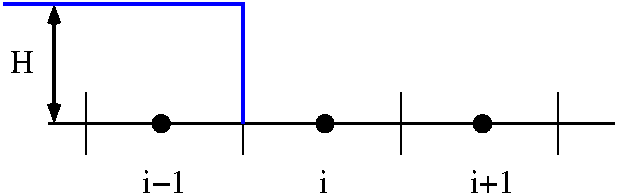
\includegraphics[width=3.0in]{calving1}  
}
\caption{Initial 1D configuration. Ice shelf with thickness $H$, with calving front at $x_{i-\half}$.}
\label{fig:initialCond}
\end{figure}

\subsection*{1D Case}
Imagine a case (Fig \ref{fig:initialCond}) where the calving front lies at the $i-\half$ face between cells ($i$) and ($i-1$); then $\phi_{i-1} = 1$ and $\phi_i=0$. (This is what things would look like immediately after the thickness-based calving law is applied, for example)

To leading order and in the absence of calving, the calving front should move at the ice velocity $U$. In the advance from time $t^n$ to time $t^{n+1} = t^n + \Delta t$, the total ice flux across the original calving front at $x_{i-\half}$ will be 
\begin{equation}
F^{n+\half}_{i-\half} = h^{n+\half}_{i-\half} U^{n}_{i-\half} \Delta t 
\label{eqn:flux}
\end{equation}
Assuming we're meeting our CFL stability constraint, the calving front will penetrate a distance of $ U^{n}_{i-\half} \Delta t < \Delta x$ into cell $i$ (Fig \ref{fig:postAdvance1D}), resulting in a new value for the ice mask $\phi$:
\begin{equation}
\phi^{*}_{i} = \frac{ U^{n}_{i-\half} \Delta t}{\Delta x}
\label{eqn:newPhi}
\end{equation}
\begin{figure}
\centerline{
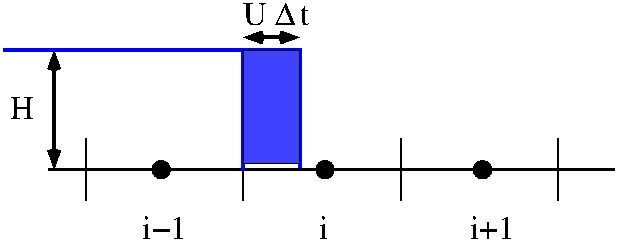
\includegraphics[width=3.0in]{calving2}  
}
\caption{1D ice shelf after advance from time $t^0$ to $(t^0 + \Delta t)$, ignoring effect of SMB and subshelf melting.  Calving front has advanced to $x_{i-\half} + U_{i-\half}\Delta t$.}
\label{fig:postAdvance1D}
\end{figure}
Ignoring any mass sources (like SMB and melting), the thickness in this portion of the cell will be $\tilde{h_i} = h^{n+\half}_{i-\half}$. However, accounting for SMB and melting, the resulting ice thickness in the partial cell will be:
\begin{equation}
\tilde{h^*_i} = h^{n+\half}_{i-\half} + \Delta t (SMB_i - b_i)
\label{eqn:newHStar}
\end{equation}
where $SMB_i$ and $b_i$ are the surface mass balance and the basal melting for cell $i$. We then can subject this to our calving criterion and convert into a cell-average value for BISICLES to carry into the next timestep:
\begin{eqnarray}
h^{n+1}_i & = & \begin{cases}
0, & if \ \  \tilde{h}^*_{i} < h_{calving} \\
 \tilde{h}^*_{i}\phi^{*}_i & otherwise 
\end{cases} 
\label{eqn:calvingLaw} \\
\phi^{n+1}_i & = & \begin{cases}
0, & if \ \  \tilde{h}^*_{i} < h_{calving} \\
 \tilde{\phi}^*_{i} & otherwise \nonumber
\end{cases} 
\end{eqnarray}
(note that there are two thickness values for the partial cell $i$:  $h_i$ is the cell-averaged thickness (over the entire cell) that we're used to thinking about, while $\tilde{h}_i$ is the thickness averaged over the ice-containing partial cell: 
\begin{eqnarray}
h_i^n & = & \frac{1}{\Delta x} \int^{x_{i+\half}}_{x_{i-\half}} h(x,t^n) dx \\
\tilde{h}^n_i & = & \frac{1}{\Delta x} \int_{x_{i-\half}}^{x_{i-\half} + \phi_i \Delta x} h(x,t^n) dx.
\end{eqnarray}

In the more general (but still 1D) case, the initial calving front position isn't necessarily at the cell face, so $(h^n_i, \phi^n_i) \ne 0$. The evolution of $\phi$ is a straightforward extension, with the additional condition that if $\phi$ increases past 1, the cell becomes a full cell.
\begin{equation}
\phi^{*}_{i} = min(1.0, \phi^n_i + \frac{ U^{n}_{i-\half} \Delta t}{\Delta x})
\label{eqn:newPhi2}
\end{equation}
To compute the new $h$, we fall back to the conservative finite-volume update, first computing the cell-averaged thickness for the entire cell using the flux through the $i-\half$ face, then computing the partial-cell ice thickness $\tilde{h}$:
\begin{eqnarray}
h_i^{*} & = & h^n_i + \Delta t U^{n}_{i-\half} h^{n+\half}_{i-\half} \\
\tilde{h}^*_{i} & = & \frac{1}{\phi^*_i}\bigl(h^*_i + \phi^*_i \Delta t (SMB_i - b_i ) \bigr) 
\end{eqnarray}
(the grouping in the second equation is descriptive of how it's actually done in the code). As before, we can then re-apply the calving criterion (eqns \ref{eqn:calvingLaw})  and then compute $h^{n+1}_i$ in the partially-filled cell.

\subsection*{2D Case}
Extending this idea to 2D, we make some assumptions and accept some inaccuracy. This is not by any means going to be as accurate as a complete embedded-boundary or levelset approach which explicitly tracks the calving front. Rather, this is primarily intended as a way to implement a simple thickness-based calving scheme in the context of MISOMIP which can allow calving-fronts to advance. I'm assuming here that as long as we have some sort of broadly physical scheme in place that the macro behavior of the system (advance or retreat) will dominate what actually occurs in these simulations.

{\bf Assumptions/design points:}
\begin{enumerate}
\item In the case of simple unidirectional flows, the method reduces to the 1D scheme just described.
\item Ice flux into partial cells is computed as usual by the finite-volume BISICLES advection update based on ice fluxes across cell faces.
\item As a first cut, assume that we also have ``area fluxes'' of $\phi$ from any upstream cells.  Once we have cell-averaged thickness and $\phi$, we can compute an ice thickness in the ice-containing part of the partial cell ($\tilde{h}^* = \frac{h^*_{ij}}{\phi^*_{ij}}$, which can then be updated as before. \footnote{This is probably the most klugey part of this. Another option could be to assume that we compute the mass fluxes and that the provisional thickness $\tilde{h}^*$ in the ice-containing part is the same thickness as the largest thickness in an upstream donor cell. There are likely other ways to approach this as well.}
\end{enumerate}
\begin{figure}
\centerline{
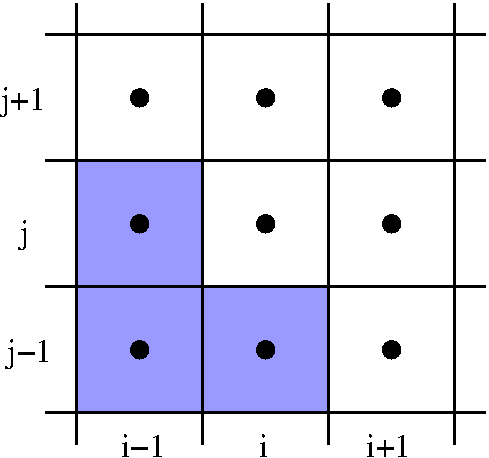
\includegraphics[width=3.0in]{calving3}  
}
\caption{Simple 2D ice shelf at time $t^0$. Calving front for cell $i$ is at faces $(i-\half,j)$ and $(i,j-\half)$.}
\label{fig:initial2D}
\end{figure}

\begin{figure}
\centerline{
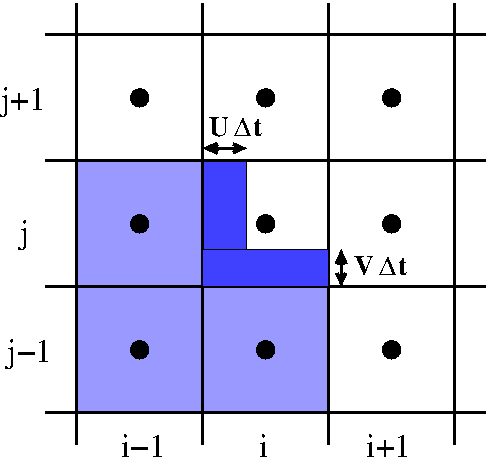
\includegraphics[width=3.0in]{calving4}  
}
\caption{2D ice shelf from Figure \ref{fig:initial2D} after advance from time $t^0$ to $(t^0 + \Delta t)$, ignoring effect of SMB and subshelf melting.  Calving front has advanced to $x_{i-\half} + U_{i-\half}\Delta t$ and $y_{j-\half} + V_{j-\half}\Delta t$}
\label{fig:postAdvance2D}
\end{figure}

For a cell $(i,j)$ which has an initial value of $\phi_{ij} < 1$ (either empty/calved or partially full), we can update as follows:
\begin{enumerate}
\item At $t^n$ we have cell-averaged thickness $h^n_{ij}$, ice fraction $\phi^n_{ij}$.
\item Compute face-centered velocities and thicknesses as usual on $x-$faces ($U^{n+\half}_{i+\half}$ and $h^{n+\half}_{i+\half}$) and on $y-$faces ($V^{n+\half}_{j+\half}$ and $h^{n+\half}_{j+\half}$).
\item Compute ice fluxes $(F_{i-\half,j}, F_{i, j-\half}) = (U_{i-\half,j}h^{n+\half}_{i-\half,j}, V_{i, j-\half}h^{n+\half}_{i, j-\half})$ \footnote{note that we have to set fluxes on cell faces between partial and empty cells to zero to prevent spurious outflow.}
\item Compute new cell-averaged $h$ and provisional $\phi$:
\begin{eqnarray} 
h^*_{ij} & = & h^n_{ij} + \frac{\Delta t}{\Delta x \Delta y}  (\Delta y F_{i-\half,j} + \Delta x F_{i,j-\half}) \\
\phi^*_{ij} & = & \phi^n_{ij} + \frac{\Delta t}{\Delta x \Delta y}(\Delta y U_{i-\half,j} + \Delta x V_{i-\half,j})  \nonumber \\
\tilde{h}^*_{ij} & = & \frac{1}{\phi^*_{ij}} \bigl( h^*_{ij} + \phi^*_{ij}\Delta t (SMB_i - b_i) \bigr) 
\end{eqnarray}

\item Apply calving criterion:
\begin{eqnarray}
h^{n+1}_{i,j} & = & \begin{cases}
0, & if \ \  \tilde{h}^*_{i,j} < h_{calving} \\
 \tilde{h}^*_{i,j}\phi^{*}_{i,j} & otherwise 
\end{cases} 
\label{eqn:calvingLaw2D} \\
\phi^{n+1}_{i,j} & = & \begin{cases}
0, & if \ \  \tilde{h}^*_{i,j} < h_{calving} \\
 \tilde{\phi}^*_{i,j} & otherwise \nonumber
\end{cases} 
\end{eqnarray}

\end{enumerate}

\section{Extension to Cliff Collapse}
We can also use this approach to implement a version of the Pollard and DeConto cliff-collapse mechanism, in which ice cliffs with a height above sea level greater than a given threshold (100m in Pollard and DeConto) experience a recession rate $r$ due to brittle failure leading to cliff collapse.

We can test for cliffs by looking for differences in surface height. For this to work properly, surface height should be computed using the effective thickness rather than the cell-centered thickness values. Since the code computes surface height $s_{i,j}$ based on cell-centered values, we can compute an effective surface height $\tilde{s}_{i,j}$ for cells in which $\phi_{i,j} < 1$:
\begin{eqnarray}
  \tilde{s}_{i,j} & = & s_{i,j} + (\tilde{h}_{i,j} - h_{i,j})  \\
  & = & s_{i,j} + h_{i,j}(\frac{1}{\phi_{i,j}} - 1) \nonumber
\end{eqnarray}

For the purposes of this model, an ice cliff is defined as a cell $(i,j)$ which meets the following conditions:
\begin{enumerate}
\item Ice in cell $(i,j)$ is grounded.
\item At least one neighbor to cell $(i,j)$ defined as open sea (zero thickness, and bed below sea level). We may wish to broaden this in the future.
\item Effective surface height is greater than the maximum cliff height: $\tilde{s}_{i,j} > s_{cliff-max}$. 
\end{enumerate}

Once a cliff has been identified, we can implement the given recession rate by reducing the area fraction of the first non-empty cell (which may or may not start the process with a full area fraction):
\begin{eqnarray}
  \phi^{new}_{i,j} & = & \phi_{i,j} - \frac{r*{\Delta t \Delta x}}{A_{i,j}} \nonumber \\
  & = &  \phi_{i,j} - \frac{r \Delta t}{\Delta x} \label{eqn:cliffCollapsePhi}
\end{eqnarray}
where $r$ is the recession rate (in $\frac{m}{a}$), $\Delta t$ is the timestep, and ${A_{i,j}}$ is the cell area (in $m$). We assume that $\tilde{h}$ is maintained through the process, meaning that the new cell-averaged thickness is given by:
\begin{eqnarray}
  h^{new}_{i,j} & = & \tilde{h}_{i,j} \phi^{new}_{i,j} \label{eqn:cliffCollapseThickness} \\
  & = & h_{i,j}\bigl(\frac{\phi^{new}_{i,j}} {\phi_{i,j}}\bigr) \nonumber
\end{eqnarray}
where $\phi_{i,j}$ and $h_{i,j}$ are the values when the cliff-collapse calving is invoked.

{\bf Implementation notes:}
\begin{enumerate}
\item For the time being, we assume the same rate of ice loss in a cliff-identified cell regardless of how many cell face directions are identified as being cliffs.
\end{enumerate}
  



\end{document}
